Eine allgemeine Systemarchitektur ist bei der Vielzahl an Paradigmen des QA nicht einfach aufzubauen. Da die ersten QA-Systeme wissensbasierte und IR-basierte Systeme sind, sind diese beiden Systeme auch die Grundlage für die Beschreibung einer allgemeinen Systemarchitektur als geeignete Kandidaten auszuweisen. 

Im Folgenden werden IR-basierte QA als Grundlage ausgewählt. Dieses hat den Zweck, um möglichst alle Komponenten der QA-Systeme abzubilden. IR-basierte QA-Systeme demonstrieren die Umwandlung von Informationen und unstrukturierten Texten, besser als wissensbasierte QA-Systeme, wo eine Abfrage einer Wissensdatenbank erfolgt. Die meisten QA-Systeme beinhalten 3 Komponenten. Diese Komponenten sind 
\begin{itemize}
\item Frage verstehen
\item Fakten extrahieren 
\item Antwort generieren
\end{itemize}




\begin{figure}[H]
    \centering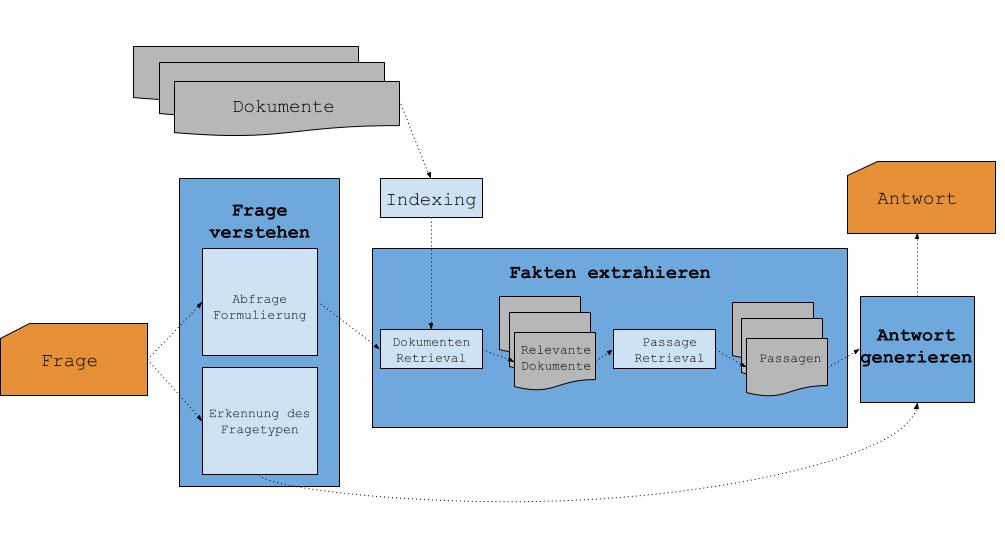
\includegraphics[width=1.0\linewidth]{images/image1.png}
    \caption[Systemarchitektur]{Systemarchitektur, in Anlehnung an \cite []{eff70}}
    \label{fig:diagram1}
\end{figure}





\section{Fragebearbeitung}

Im ersten Modul eines QA-Systems geht es darum, die gestellte Frage zu verstehen. Zunächst muss die in natürlicher Sprache gestellten Frage in eine Abfrage umgewandelt werden, welches ein Computer versteht. Außerdem wird in diesem Modul der Typ der gestellten Frage festgelegt um die Auswahl der Antwortkandidaten, welches im letzten Modul eines QA-Systems stattfindet, zu begrenzen.

\subsection{Abfrageformulierung}
Zunächst muss die gestellte Frage in eine Abfrage übersetzt werden, welches der Computer verstehen kann. Bei einer Suchmaschine etwa, wird die Frage in natürlicher Sprache gestellt, jedoch muss der Computer im Hintergrund diese Abfrage in eine Datenbankabfrage umwandeln. 
\textbf{LIN 2007} zeigt wie man mittels  \enquote{Query Reformulation} die gestellte Frage reformuliert, also nicht mehr als Frage, sondern als Aussage wiedergibt. Dabei werden vordefinierte Regeln verwendet. Dieses ist nützlich, denn Textausschnitte aus dem Web können unterschiedlich formuliert sein.

\subsection{Antworttypen}

Durch Named Entitiy Recognition ist es möglich, die gestellte Frage nach seinem Typ zu kategorisieren. Eine \enquote{Wer-Frage} wird dabei mit Person verknüpft eine \enquote{Wo-Frage} mit dem Ort. Diese Klassifizierung ermöglicht dem System eine Vorselektion durchzuführen. 

Eine \enquote{Taxonomie} von Antworttypen kann aus dem WordNet, wie in den Beispielen \textbf{HARBAYAIN, PASCA}, gebildet werden.

Im Beispiel von \textbf{Li and Roth 2005} sieht man, wie solche Taxonomien selbst gemacht werden können, also ohne WordNet. Die Granularität dieser Taxonomien kann dabei selbst bestimmt werden. Die Entität PERSON kann dabei viel tiefer behandelt werden, also PERSON:GRUPPE. 


\section{Abrufen von Dokumenten und Passagen}
Die aus der Fragenbearbeitungsphase erzeugte IR-Abfrage wird an eine IR-Engine gesendet.
Dies führt zu einer Reihe von Dokumenten, die nach ihrer Relevanz für die Abfrage geordnet sind. Da die meisten Methoden zum Extrahieren von Antworten für kleinere Bereiche wie Absätze ausgelegt sind, unterteilen QA-Systeme als Nächstes die obersten n Dokumente in kleinere Passagen wie z.B. Abschnitte, Absätze oder Sätze. 


Die einfachste Form des Passagen Retrievals besteht darin, jede Passage zur Stufe der Antwortextraktion weiterzuleiten. Eine komplexere Variante besteht darin, die Passagen zu filtern, indem eine benannte Entität oder eine Antworttypklassifizierung für die abgerufenen Passagen ausgeführt wird, wobei Passagen verworfen werden, die nicht den Antworttyp der Frage enthalten. Es ist auch möglich, überwachtes Lernen zu verwenden, um die verbleibenden Passagen mithilfe von Funktionen wie:

\begin{itemize}
\item Die Anzahl der benannten Entitäten des richtigen Typs in der Passage
\item Die Anzahl der Frage-Schlüsselwörter in der Passage 
\item Die längste exakte Folge von Frage-Schlüsselwörtern, die in der Passage vorkommt
\item Der Rang des Dokuments, aus dem die Passage extrahiert wurde
\item Die Nähe von die Schlüsselwörter aus der ursprünglichen Abfrage untereinander (Pasca 2003, Monz 2004).
\item Die Anzahl der n-Gramm, die sich zwischen der Passage und der Frage überlappen (Brill et al., 2002).
\end{itemize}

\section{Antwortextraktion}
Die letzte Phase der Beantwortung von Fragen besteht darin, eine bestimmte Antwort aus der Passage zu extrahieren, z. B. auf eine Frage wie „Wie hoch ist der Berg? Everest?" die Höhenangabe zu geben. Diese Aufgabe wird üblicherweise durch Beschriftung modelliert. 
Ein einfacher Algorithmus für die Antwortextraktion besteht darin, einen Entitäts-Tagger in der Kandidatenpassage auszuführen und die passende Passage zurückzugeben, die den richtigen Antworttyp enthält. 
In den folgenden Beispielen würden die unterstrichenen benannten Entitäten aus den Passagen als Antwort auf die Fragen HUMAN und DISTANCE-QUANTITY extrahiert:

\newtheorem{example}{Beispiel}

\begin{example}
\enquote{Wer ist der indische Premierminister?} - \textbf{Manmohan Singh}, Premierminister von Indien, hatte den linken Führern gesagt, dass das Abkommen nicht neu verhandelt werden würde.

\end{example}
\begin{example}
\enquote{Wie hoch ist der Berg Everest?} - Die offizielle Höhe des Mount Everest beträgt \textbf{29029 Fuß}.
\end{example}

Leider sind die Antworten auf viele Fragen, wie z. B. DEFINITION-Fragen, in der Regel nicht von einem bestimmten benannten Entitätentyp. Aus diesem Grund verwendet die moderne Arbeit zur Antwortextraktion komplexere Algorithmen, die im Allgemeinen auf überwachtem Lernen basieren. Im nächsten Abschnitt wird ein einfacher merkmalsbasierter Klassifikator vorgestellt. Anschließend wenden wir uns modernen neuronalen Algorithmen zu.